\documentclass[journal]{IEEEtran}

\usepackage{graphicx}
\usepackage{natbib}

\title{Integrating Solar on the Grid}
\author{Aidan Sharpe}

\begin{document}
	\maketitle
	\begin{abstract}
		Solar power is becoming more popular every year. Whether it be domestic rooftop panels or an acres-large array, they seem to be on the forefront of renewable electricity. However, there is one thing that puts solar panels apart from almost all other forms of electricity production -- a direct current (DC) output. This difference, while small at first glance, introduces a plethora of engineering challenges to make solar play nicely with the electric grid. 
	\end{abstract}

	\section{Introduction}
	\IEEEPARstart{D}{epending} on who you ask, solar energy is either an incredible technology that will save the planet, an over-hyped technology that rarely comes up net-carbon zero, or a technology that is really cool in concept but involves doing lots of complicated math. Regardless, when most people think of solar energy, dark blue photo-voltaic (PV) cells often come to mind. While there are several less common forms of solar electricity generation, this is by far the most common. But how do they work, and how can they be incorporated into an electric grid?
	
	The most important part of understanding any system is getting a surface-level conceptual feel for it. When it comes to solar power on the grid there are a few fundamentals to grasp before diving head-first into math and models. First and foremost, what is a photo-voltaic cell? Etymologically speaking, \textit{"photo"} generally means \textit{with light}, \textit{"voltaic"} has to do with voltage -- a potential to do work with electricity, and a \textit{"cell"} is a small, usually repeating, unit. Therefore, a photo-voltaic cell is a unit that can use light to do work. From a technical standpoint, this is an accurate yet not complete description. It is important to note that the voltage created by a PV cell is nearly constant, and therefore would result in a direct current.
	
	The same surface-level, conceptual understanding of an electric grid is also important. In North America, the power grid is 120 root mean squared (RMS) volts at 60 hertz. The RMS, a type of averaging technique, of any signal can be found using equation \ref{eq:rms}. However, when the signal is a pure sine wave, like it is on the power grid, it can be found simply by dividing the peak amplitude of the voltage by $\sqrt{2}$. Additionally, since a sine wave is cyclical in nature, it is commonly the case that angular frequency, signified by an $\omega$, is preferred. This angular frequency can be found simply by multiplying the frequency by $2\pi$. The final important component of a power grid is known as phase-shift. Denoted by an angle, $\phi$, phase-shift is basically a measure of how lined up the voltage signal and current signal are. In the case of a power grid, the closer this angle is to 0, the better. The effects of the different variables can be seen in figure \ref{fig:acpower}.
	% RMS of a function over a time period
	\begin{equation}
		\label{eq:rms}
		f_{RMS}=\sqrt{\frac{1}{T_2 - T_1}\int_{T_1}^{T_2}[f(t)] ^2 dt}
	\end{equation}
	
	%image of ac power functions
	\begin{figure}
		\centering
		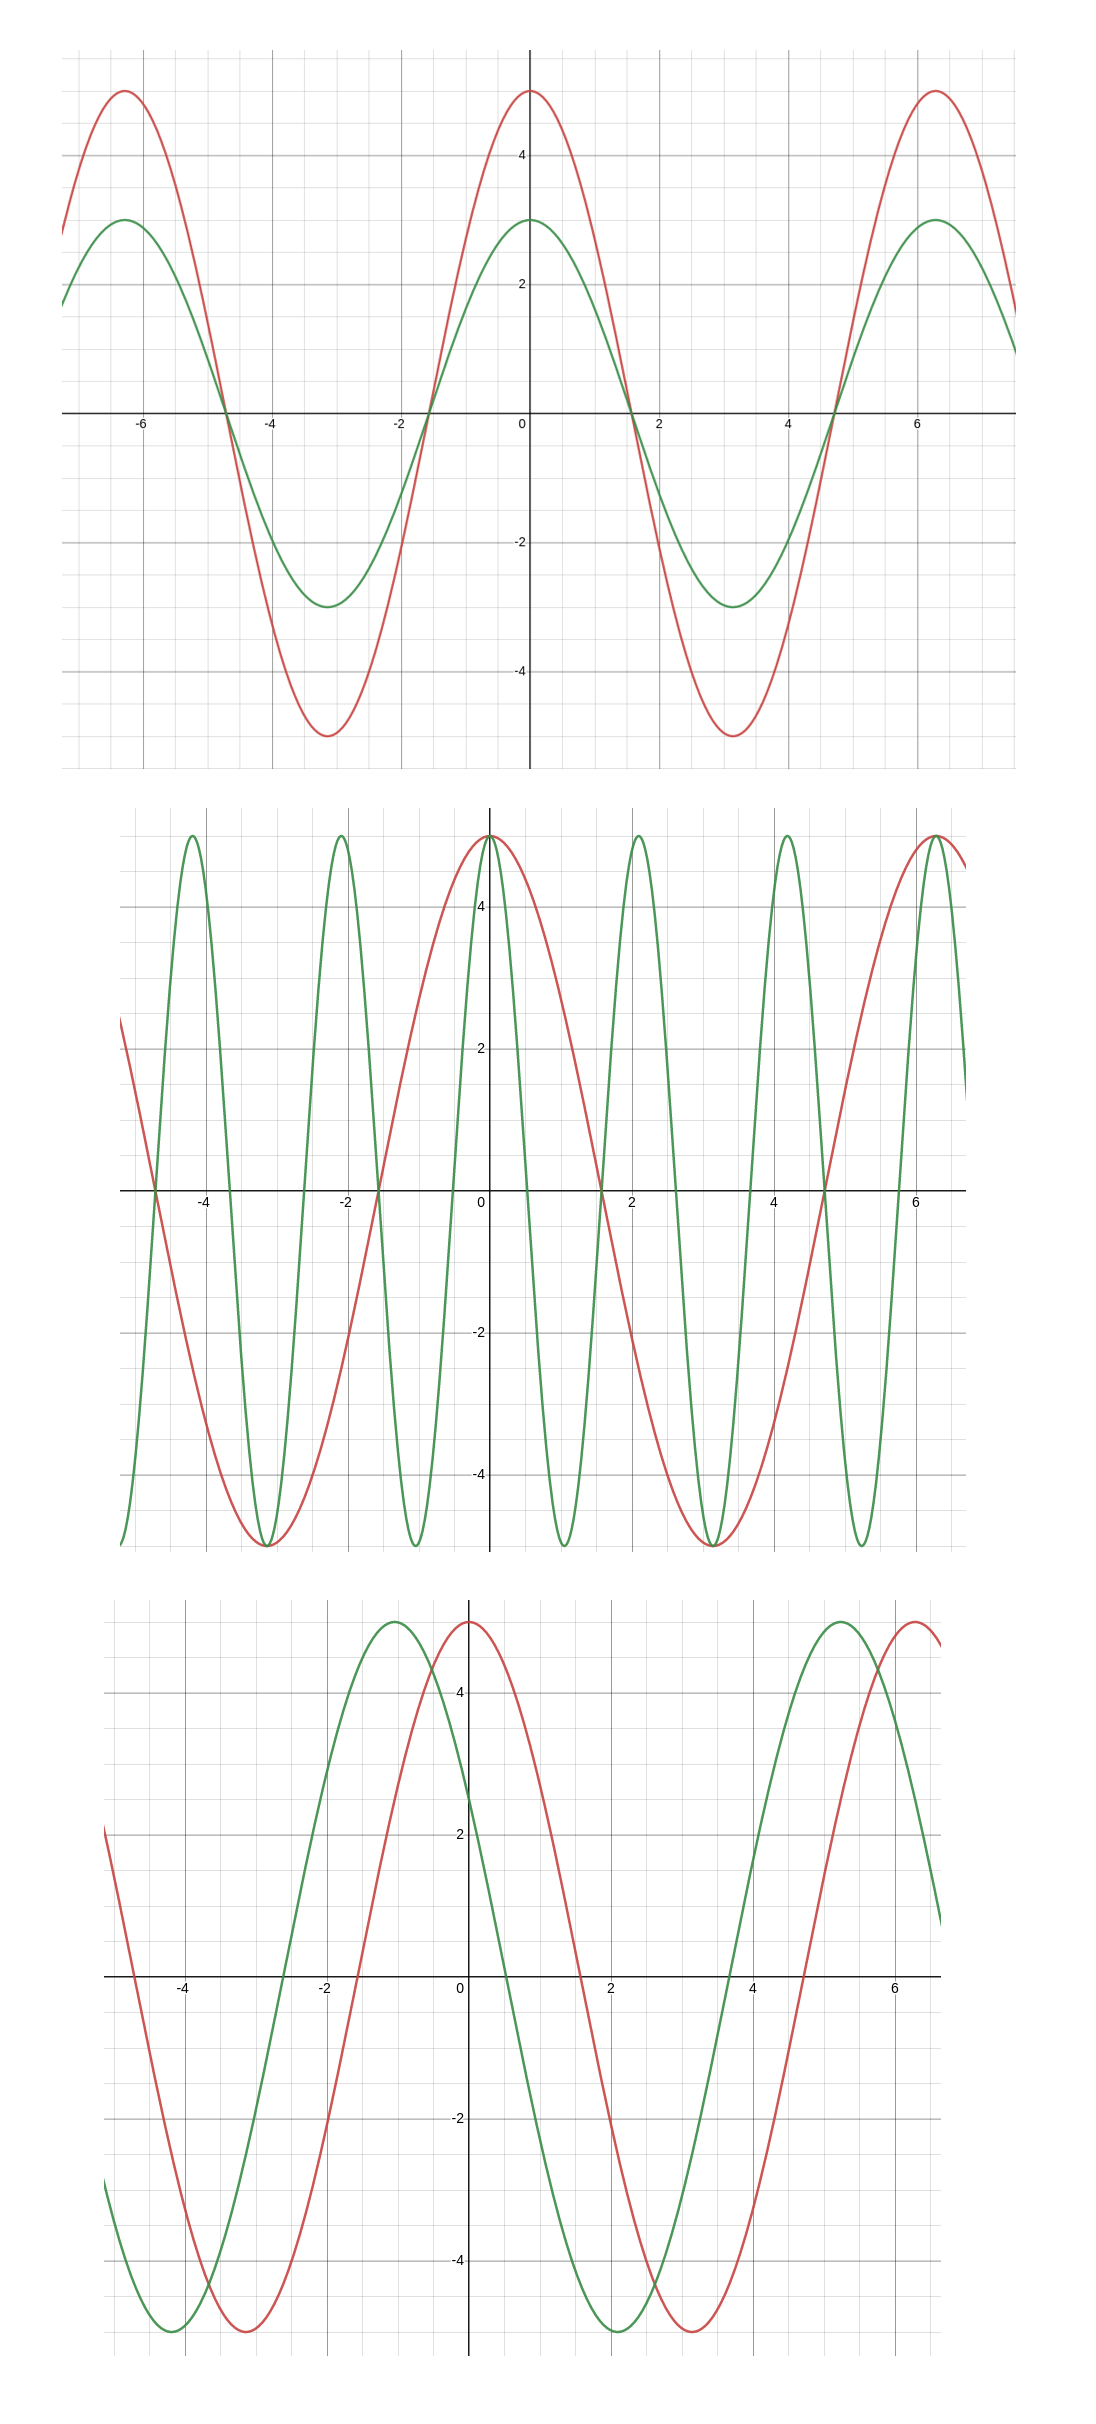
\includegraphics[scale=0.6]{ACShifts.png}
		\caption{How amplitude, frequency, and phase-shift affect a function}
		\label{fig:acpower}
	\end{figure}

	\section{How do PV Cells Work?}
	How do photo-voltaic cells \textit{actually} create a voltage with light? The absorption of light creates a voltage due to the photovoltaic effect. What is that? First observed in 1839 by French physicist, Alexandre Edmond Bequerel, when he detected a sunlight induced voltage between two pieces of metal in hydrochloric acid, the photovoltaic effect describes certain conditions that create measurable voltages from photons \citep{Yang2019}.
	
	In 1954, a team of researchers at Bell Labs in New Jersey invented the silicon solar cell \citep{Yang2019}. Today, solar cells are almost universally made from semiconducting materials, as light can easily cause the movement of electrons in them \cite{Luque2011}.
	Silicon, known today for its prevalence in the computing industry, is a semi-conducting metalloid. 
	
	Modern solar panel operate on the following principle: when exposed to light a connection between silicon with positively charged impurities and silicon with negatively charged impurities creates a DC voltage \citep{Luque2011}.
	
	\section{How does the Grid Work?}
	On the contrary, the power grid runs on alternating current (AC). As summarized earlier, there are three primary variables used to define an AC signal: amplitude (A), angular frequency ($\omega$), and phase-shift ($\phi$). Almost any AC signal can be written in the form shown by equation \ref{eq:ac}. 
	\begin{equation}
		\label{eq:ac}
		f(t) = A\cos(\omega t + \phi)
	\end{equation}

	The reason power grids the world over use AC rather than DC has do with minimizing power loss. As seen in equation \ref{eq:pwrLoss}, power lost is inversely proportional to the square of the input voltage. Therefore, increasing the input voltage will aid in reducing the amount of power lost to the grid. 
	
	AC shines in this case simply because of how easy and inexpensive it is to increase and decrease voltage. As seen in figure \ref{fig:transformer} AC voltage can be increased by many orders of magnitude with minimal power loss simply by passing it through a step up transformer: a circuit comprised of little more than a bunch of coils of wire. This circuit acts like a first class lever for electricity. On the other hand, DC voltage requires much more complex circuitry to achieve even small amounts of voltage increase. 
	%image of transformer
	\begin{figure}[h]
		\centering
		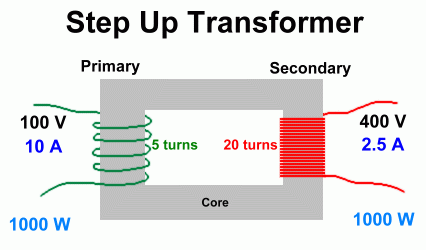
\includegraphics[scale=0.4]{step-up-transformer.png}
		\caption{Step up transformer \citep{Transformer}}
		\label{fig:transformer}
	\end{figure}
	
	\begin{equation}
		\label{eq:pwrLoss}
		P_{loss} = \frac{\rho L}{A} \left( \frac{P_{initial}}{V} \right) ^2
	\end{equation}

	Importantly, the grid is very picky. For the safety of both grid workers and those using it, the power supplied to the grid must exactly match the current power demand. Additionally, the voltage supplied must always be the same and in phase with the current supplied, and the frequency must not vary. If any of these requirements are not met, the safety and reliability of the grid become compromised. Therefore, precautions must be put into place to make sure that voltage is constant and in-phase.
	
	\section{DC Sources on an AC Grid}
	For two reasons, ensuring the safety and reliability of the grid becomes difficult when attempting to add a DC supply. First, DC power must be converted to AC power, requiring complex circuitry. Second, communication between all power grid providers must be clear and established to ensure that only the appropriate amount of power is delivered. 
	
	Anyone who has ever powered an appliance off of a car battery has used a DC to AC inverter. While these are much smaller scale than grid-interactive inverters, they often fulfill a quite similar function. A grid-tied DC supply will use a grid-interactive inverter to perform its task. These tasks include: converting DC power to AC power, ensuring that proper voltage and frequency are being created, making sure that power is optimized, and protecting itself and the power grid \citep{Stapleton2011}. 
	
	When inverters are used to provide grid power, they must first pass power through a switchboard. The role of the switchboard is to monitor the system and electrically isolate inverter from the grid in the event of an emergency to prevent power surges and provide general protection \citep{Stapleton2011}. A model of the system is seen in figure \ref{fig:domestic}.
	
	% image of domestic setup
	\begin{figure}[h]
		\centering
		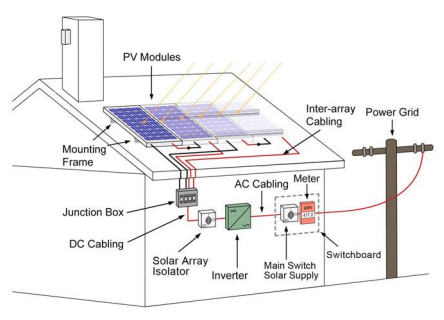
\includegraphics[scale=0.45]{DomesticSolarModel.png}
		\caption{Model of domestic grid-enabled solar system \citep{Stapleton2011}}
		\label{fig:domestic}
	\end{figure}
	\section{Conclusions}
	While supplying the grid with domestic solar power has many complex parts, it is certainly the case that the technology is quite mature. When it comes to adding solar to homes, there are a wide number of options available for consumers and businesses. Large power banks for domestic use might not yet be at the point where they are cheap and sustainable, but they are publicly available nonetheless. 
	
	In the coming years, renewable energy will likely be at the forefront of electrical engineering. Going forward, energy production is probably going to become more local as more and more people adopt at-home alternatives. Manufacturing techniques and broader understanding of incorporating domestic PV arrays on the grid are driving prices down. The day is fast approaching, where a combination of solar and power is more economical than strictly grid power.
	\bibliography{bib}
	\bibliographystyle{ieeetr}	
\end{document}